%%%%%%%%%%%%%%%%%%%%%%%%%%%%%%%%%%%%%%%%%
% Beamer Presentation
% LaTeX Template
% Version 1.0 (10/11/12)
%
% This template has been downloaded from:
% http://www.LaTeXTemplates.com
%
% License:
% CC BY-NC-SA 3.0 (http://creativecommons.org/licenses/by-nc-sa/3.0/)
%
%%%%%%%%%%%%%%%%%%%%%%%%%%%%%%%%%%%%%%%%%

%----------------------------------------------------------------------------------------
%	PACKAGES AND THEMES
%----------------------------------------------------------------------------------------

%\documentclass[handout]{beamer}
\documentclass{beamer}

\mode<presentation> {

% The Beamer class comes with a number of default slide themes
% which change the colors and layouts of slides. Below this is a list
% of all the themes, uncomment each in turn to see what they look like.

%\usetheme{default}
%\usetheme{AnnArbor}
%\usetheme{Antibes}
%\usetheme{Bergen}
%\usetheme{Berkeley}
%\usetheme{Berlin}
%\usetheme{Boadilla}
\usetheme{CambridgeUS}
%\usetheme{Copenhagen}
%\usetheme{Darmstadt}
%\usetheme{Dresden}
%\usetheme{Frankfurt}
%\usetheme{Goettingen}
%\usetheme{Hannover}
%\usetheme{Ilmenau}
%\usetheme{JuanLesPins}
%\usetheme{Luebeck}
%\usetheme{Madrid}
%\usetheme{Malmoe}
%\usetheme{Marburg}
%\usetheme{Montpellier}
%\usetheme{PaloAlto}
%\usetheme{Pittsburgh}
%\usetheme{Rochester}
%\usetheme{Singapore}
%\usetheme{Szeged}
%\usetheme{Warsaw}

% As well as themes, the Beamer class has a number of color themes
% for any slide theme. Uncomment each of these in turn to see how it
% changes the colors of your current slide theme.

%\usecolortheme{albatross}
\usecolortheme{beaver}
%\usecolortheme{beetle}
%\usecolortheme{crane}
%\usecolortheme{dolphin}
%\usecolortheme{dove}
%\usecolortheme{fly}
%\usecolortheme{lily}
%\usecolortheme{orchid}
%\usecolortheme{rose}
%\usecolortheme{seagull}
%\usecolortheme{seahorse}
%\usecolortheme{whale}
%\usecolortheme{wolverine}

%\setbeamertemplate{footline} % To remove the footer line in all slides uncomment this line
%\setbeamertemplate{footline}[page number] % To replace the footer line in all slides with a simple slide count uncomment this line

%\setbeamertemplate{navigation symbols}{} % To remove the navigation symbols from the bottom of all slides uncomment this line
}



\setbeamertemplate{itemize items}[default]
\setbeamertemplate{enumerate items}[default]

\usepackage{pgfpages}
\usepackage{graphicx} % Allows including images
\usepackage{booktabs} % Allows the use of \toprule, \midrule and \bottomrule in tables
\usepackage{tikz}

%\pgfpagesuselayout{16 on 1}[a4paper,landscape,border shrink=0mm]

%----------------------------------------------------------------------------------------
%	TITLE PAGE
%----------------------------------------------------------------------------------------

\title[]{Learning Rules With Numerical and Categorical
Attributes from Linked Data Sources} % The short title appears at
%the bottom of every slide, the full title is only on the title page

\author{Andre de Oliveira Melo} % Your name
\institute[Saarland University] % Your institution as it will appear on the bottom of every slide, may be shorthand to
%save space
{
Saarland University \\ % Your institution for the title page
\medskip
\textit{andresony@gmail.com} % Your email address
}
\date{\today} % Date, can be changed to a custom date

\begin{document}

\begin{frame}
\titlepage % Print the title page as the first slide
\end{frame}

\begin{frame}
\frametitle{Overview} % Table of contents slide, comment this block out to remove it
\tableofcontents % Throughout your presentation, if you choose to use \section{} and \subsection{} commands, these will automatically be printed on this slide as an overview of your presentation
\end{frame}

%----------------------------------------------------------------------------------------
%	PRESENTATION SLIDES
%----------------------------------------------------------------------------------------

%------------------------------------------------
\section{Introduction}
%------------------------------------------------

\begin{frame}
\frametitle{Semantic Web}

\begin{block}{Semantic Web}
  \begin{quote}
    ``provides a common framework that allows data to be shared and reused across application, enterprise, and community
    boundaries''
  \end{quote}
\end{block}
\pause
\begin{block}{Linked Data}
  % \begin{quote}
  % ``a term used to describe a recommended best practises for exposing, sharing, and connecting pieces of data,
  %information and knowledge on the Semantic Web using URIs and RDF''
  %\end{quote}
  \begin{quote}
  ``collection of interrelated datasets on the Web''
  \end{quote}
  \begin{quote}
  ``recommended best practises for exposing, sharing, and connecting pieces of data, information and knowledge on the
Semantic Web''
  \end{quote}
\end{block}
\end{frame}
%------------------------------------------------
\begin{frame}
  \begin{figure}
  \includegraphics[width=1\linewidth]{./Figures/lod-datasets_2011-09-19}
  \end{figure}
\end{frame}
\begin{frame}
  \begin{figure}
  \includegraphics[width=1\linewidth]{./Figures/lod-zoomed2}
  \end{figure}
\end{frame}
%-----------------------------------------------------------------------------------------------------------------------
\section{Motivation}
%-----------------------------------------------------------------------------------------------------------------------
\begin{frame}
\frametitle{Motivation}
Learn Datalog rules from data:
\begin{center}
  $\underbrace{livesIn(X,Y)}_{head}$ :- $\underbrace{isMarriedTo(X,Z),livesIn(Z,Y)}_{body}$
\end{center}
Support and confidence thresholds
\begin{itemize}
 \item Support: $supp(head$ :- $body)=supp(head \wedge body)$
 \item Confidence: $conf(head$ :- $body)=\cfrac{supp(head \wedge body)}{supp(body)}$ 
\end{itemize}
\end{frame}
%-----------------------------------------------------------------------------------------------------------------------
\begin{frame}
\frametitle{Rules with constants}
  Refining rules with constants is relevant
  \begin{center}
     $speaks(X,Z)$ :- $livesIn(X,W)$
  \end{center}

  Searching constants for $Z$ and $W$ we can learn:
  \begin{align*}
    speaks(X,englsih)&\text{ :- }livesIn(X,australia) \\
    speaks(X,spanish)&\text{ :- }livesIn(X,argentina) \\
    speaks(X,portuguese)&\text{ :- }livesIn(X,brasil)
  \end{align*}

  What about numerical constants?
  \begin{align*}
    speaks(X,english)&\text{ :- }hasIncome(X,\$3.71Billion) \\
    speaks(X,portuguese)&\text{ :- }livesIn(X,W),hasPopulation(W,193946886)
  \end{align*}
\end{frame}
%-----------------------------------------------------------------------------------------------------------------------
\begin{frame}
\frametitle{Refining rules with numerical intervals}
 \emph{maritalStatus(X, single) :- age(X,Y)} [conf=0.40]\\
 \emph{maritalStatus(X,married) :- age(X,Y)} [conf=0.46]\\
 \emph{maritalStatus(X,widowed) :- age(X,Y)} [conf=0.06]
 \begin{columns}[c]
    \column{0.33\textwidth}
      \center Single
      \begin{figure}
      \includegraphics[width=1\linewidth]{./Figures/age-single.png}
      \end{figure}
    \column{0.33\textwidth}
      \center Married
      \begin{figure}
      \includegraphics[width=1\linewidth]{./Figures/age-married.png}
      \end{figure}
    \column{0.33\textwidth}
     \center  Widowed
      \begin{figure}
      \includegraphics[width=1\linewidth]{./Figures/age-widowed.png}
      \end{figure}
  \end{columns}
\end{frame}
%-----------------------------------------------------------------------------------------------------------------------
\begin{frame}
\frametitle{Combine with categorical constants}
  For $maritalStatus(X,married$), $minConf=0.75$ is not satisfied. \\
  Refine by State? 

  \begin{columns}[c]
   \column{0.45\textwidth}
      \center USA
      \begin{figure}
      \includegraphics[width=1\linewidth]{./Figures/age-married-minConf.png}
      \end{figure}
  \column{0.1\textwidth}
      $\Rightarrow$
   \column{0.45\textwidth}
      \center South Dakota
      \begin{figure}
      \includegraphics[width=1\linewidth]{./Figures/age-married-southdakota-minConf.png}
      \end{figure}
  \end{columns}
\end{frame}
%-----------------------------------------------------------------------------------------------------------------------
\begin{frame}
\frametitle{Combine with categorical constants}      
  We can find intervals for $Y$ that satisfy $minConf=0.75$ for \emph{maritalStatus(X,widowed) :-
livesIn(X,sd),age(X,Y)} and...
  \begin{figure}
  \includegraphics[width=0.8\linewidth]{./Figures/usmap.png}
  \end{figure}

\end{frame}
%-----------------------------------------------------------------------------------------------------------------------
\begin{frame}
\frametitle{Base-rule and Refined-rule}
  \begin{itemize}
   \item \textbf{Base-rule}: Numerical argument with no constant \\
      $r_1: marritalStatus(X,single)$ :- $livesIn(X,sd),age(X,Y)$ \\ 
      \quad \quad [conf=0.49,supp=2368]
   \item \textbf{Refined-rule}: Base-rule with restricted numerical variable \\  
      $r_2: marritalStatus(X,single)$ :- $livesIn(X,sd),age(X,Y),Y\in[33,67]$ \\ 
      \quad \quad [conf=0.77,supp=1092]
  \end{itemize}
 We are interested in refinements that bring a significant confidence gain:
 \begin{equation}
  gain_{r_{ref},r_{base}}=\cfrac{conf(r_{ref})}{conf(r_{base})}
 \end{equation}
 For our example:
 \begin{math}
  gain_{r_{2},r_{1}}=\cfrac{0.77}{0.49}=1.57
 \end{math}
\end{frame}
%-----------------------------------------------------------------------------------------------------------------------
\begin{frame}
 How can we obtain high confidence gain?
 \begin{itemize}
  \item Satisfy support threshold
  \item Do not necessarily satisfy confidence threshold
  \item Potentially has a refined-rule with an interval that satisfies both thresholds \\
    \quad i.e., has non-uniform confidence distribution along the numerical attribute\\
    \quad i.e., has body support and positives (body$\wedge$head) support distributions are different
 \end{itemize}
\end{frame}
%-----------------------------------------------------------------------------------------------------------------------
\begin{frame}
\frametitle{Motivation}
 Example for a rule with positives support 117 and body support 700:
\begin{columns}[c]
  \column{0.45\textwidth}
    \begin{figure}
    \includegraphics[height=0.3\textheight]{./Figures/supportDistribution}
    \end{figure}
    \begin{figure}
    \includegraphics[height=0.3\textheight]{./Figures/probabilityDistribution}
    \end{figure}
  \column{0.1\textwidth}
    %\begin{centerline}
      %\begin{fontsize}{20}{24}$\rightarrow$\end{fontsize}
      $\rightarrow$
    %\end{centerline}
  \column{0.45\textwidth}
    \begin{figure}
    \includegraphics[width=1\linewidth]{./Figures/confidenceDistribution}
    \end{figure}
\end{columns}

\end{frame}
%-----------------------------------------------------------------------------------------------------------------------
\begin{frame}
\frametitle{Motivation}
 Problem?
 \begin{itemize}
    \item Search space grows exponentially with the number of predicates and constants
    \item Querying support and confidence distributions is very expensive
 \end{itemize}
 Idea:
 \begin{itemize}
    \item Analyze combinations of numerical and categorical properties
    \item Measure their level of interestingness
    \item Use core-ILP algorithm
    \item Extend it to focus on most interesting combinations
 \end{itemize}
\end{frame}
%-----------------------------------------------------------------------------------------------------------------------
\section{Inductive Logic Programming}
%-----------------------------------------------------------------------------------------------------------------------
\begin{frame}
\frametitle{ILP}
 Inductive Logic Programming: Finds a hypothesis $\mathcal{H}$ that covers all positive, and no negative examples
  \begin{fontsize}{10}{10}
    \begin{center}
    $positiveExamples + negativeExamples + background Knowledge \rightarrow hypothesis$
    \end{center}

    \begin{table}
      \begin{tabular}{ l  l }
      \toprule
      \textbf{Training Examples} & \textbf{Background Knowledge}\\
      \midrule
      daughter(mary,ann) +	& parent(ann,mary)	\\
      daughter(eve,tom)  +	& parent(ann, tom)	\\
      daughter(tom,ann)  - 	& parent(tom,eve)	\\
      daughter(eve,ann)  -	& parent(tom,ian) 	\\
				& female(ann)		\\
				& female(mary)		\\
				& female(eve)		\\
      \bottomrule
      \end{tabular}
    \end{table}
    \begin{center}
      $\mathcal{H} = daughter(X,Y)$ :- $female(X),parent(Y,X)$ 
    \end{center}


  \end{fontsize}
\end{frame}
%-----------------------------------------------------------------------------------------------------------------------
\begin{frame}
\frametitle{Logic Programming Concepts}
  \begin{itemize}
   \item Literal: predicate symbol with bracketed n-tuple, e.g: \\ 
      \quad $L=livesIn(X,Y)$
   \item Clause: a disjunction of literals (negated or not), e.g: \\ 
      \quad $c=(L_1 \vee L_2 \vee \ldots \vee \neg L_{m-1} \vee \neg L_{m})$
   \item Safe Datalog Rules: Every variable in the head appear in a non-negated literal in the body, negated literal
variables in the body should appear in some positive literal in the body, e.g.: \\ 
    \quad $speaks(X,Y)$ :- $wasBornIn(X,Z),hasOfficialLanguage(Z,Y)$
   \item Hypothesis: a set of clauses $\mathcal{H}$
     \begin{itemize}
	\item Completeness: $\mathcal{H}$ covers all positive examples
	\item Consistency: $\mathcal{H}$ covers no negative examples
     \end{itemize}
  \end{itemize}
\end{frame}
%-----------------------------------------------------------------------------------------------------------------------
\begin{frame}
\frametitle{ILP}
Approaches
  \begin{itemize}
   \item Bottom-up: Start with least general $\mathcal{H}$ then perform generalizations
   \item \textbf{Top-down}: Start with most general $\mathcal{H}$ then perform specializations
   \begin{itemize}
    \item Specialization loop: adds literals to a clause and ensures consistency
    \item Covering loop: adds clauses to the hypothesis and ensures completeness
    \item Apriori-style pruning
   \end{itemize}
  \end{itemize}
What about large, noisy and incomplete LOD datasets such as YAGO and DBpedia?:
\begin{itemize}
   \item Sample data to reduce size
   \item Restrict the number of literals in a clause
   \item Tolerate a certain level of inconsistency and incompleteness \\ \quad
      Expected Accuracy:  $A(c)=P(e \in \mathcal{E}^{+}|c)=\cfrac{n^{+}(c)}{n^{+}(c)+n^{-}(c)}$
  \end{itemize}
\end{frame}
%-----------------------------------------------------------------------------------------------------------------------
\section{Learning Rules With Numerical and Categorical Attributes}
%-----------------------------------------------------------------------------------------------------------------------
\begin{frame}
\frametitle{Correlation between Literals}
Let's say we want to refine a clause with $hasIncome(X,Y)$ with an interval for $Y$.
Refine by $quarterOfBirth$ or $hasEducation$?
\begin{columns}[c]
  \column{0.5\textwidth}
    \begin{fontsize}{7}{8}
      \center{$hasIncome(X,Y),quarterOfBirth(X,Z)$}
    \end{fontsize}
    \begin{figure}
    \includegraphics[width=1\linewidth]{./Figures/income-birthquarter-zoom.png}
    \end{figure}
  \column{0.5\textwidth}
    \begin{fontsize}{7}{8}
      \center{$hasIncome(X,Y),hasEducation(X,Z)$}
    \end{fontsize}
    \begin{figure}
    \includegraphics[width=1\linewidth]{./Figures/income-education-zoom.png}
    \end{figure}
\end{columns}
\end{frame}
%-----------------------------------------------------------------------------------------------------------------------
\begin{frame}
\frametitle{Correlation between Literals}
  \begin{columns}[c]
    \column{0.75\textwidth}
      \begin{figure}
      \includegraphics[width=0.9\linewidth]{./Figures/prof-nurs.png}
      \end{figure}
    \column{0.25\textwidth}
	\begin{table}\tiny
	  \begin{tabular}{l}
	    \toprule
	    \textbf{Educational Levels} \\
	    \midrule
	    Nursery school to grade 4 \\
	    Grade 5 or grade 6 \\
	    Grade 7 or grade 8 \\
	    Grade 9	 \\
	    Grade 10 \\
	    Grade 11 \\  
	    Grade 12 no diploma \\
	    High school graduate\\
	    Some college ($<$ 1 year) \\
	    Some college ($\geq$ 1 year) \\
	    Associate's degree \\
	    Bachelor's degree \\
	    Master's degree \\
	    Professional school degree \\
	    Doctorate degree \\
	    \bottomrule	
	\end{tabular}
      \end{table}
  \end{columns}
\end{frame}
%-----------------------------------------------------------------------------------------------------------------------
%\begin{frame}
%\frametitle{Correlation between Literals}
%  \begin{figure}
%  \includegraphics[width=1\linewidth]{./Figures/income-education.png}
% \end{figure}
%\end{frame}
%-----------------------------------------------------------------------------------------------------------------------
\begin{frame}
\frametitle{Interestingness Measure}
  How to measure of the interestingness of adding a literal $l$ to a clause $c$?
  \begin{itemize}
   \item Extract the probability distribution of $\{c\}$ and $\{c \wedge l\}$ along $Y$
   \item Normalize both support distributions and measure their divergence (e.g., with Kullback-Leibler)
  \end{itemize}
  But, divergence alone isn't a good idea because:
  \begin{itemize}
   \item Lower support histograms are more likely to have a divergent distribution (\emph{sampling error})
   \item Rules with high support are still interesting
  \end{itemize}
  Then combine both measures: divergence*support
\end{frame}
%-----------------------------------------------------------------------------------------------------------------------
\begin{frame}
\frametitle{Correlation Lattice}
  \begin{itemize}
   \item Build a lattice similar to an itemset lattice 
   \item Numerical property $r$ as root 
   \item The ``items'' are literals that can be joined with the root's non-numerical variable $X$
   \item Root's numerical attribute domain is discretized in $k$ buckets $b_1,\dots,b_k$
   \item Each node $x$ has a frequency histogram $h(x)=<h_1(x),\ldots,h_k(x)>$ from its clause support distribution \\
      \quad where $h_i(x)=supp(x|Y \in b_i)$ \quad and \quad $|h(x)|_1=supp(x)$
   %\item Then we can use it to suggest the most interesting literals to be added in the refinement step from core-ILP
   %\item Idea is to generate a correlation lattice for each numerical attribute as preprocessing step 
  \end{itemize}
\end{frame}
%-----------------------------------------------------------------------------------------------------------------------
\begin{frame}
 \frametitle{Correlation Lattice}
  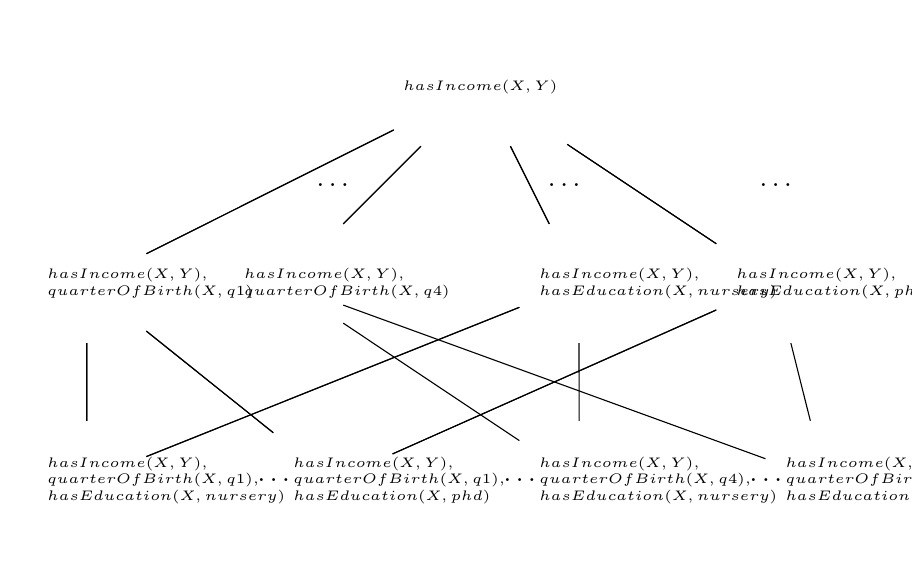
\begin{tikzpicture}[scale=1.25,auto=center,every node/.style={,minimum size=1.5cm,font=\tiny}]
    \node (r) 	at (5,5)  {$hasIncome(X,Y)$};
    \pause
    
    \node[rectangle,text width=1cm,align=center] (a1) 	at (1,3) {$hasIncome(X,Y),$\\$quarterOfBirth(X,q1)$};
    \node[rectangle,text width=1cm,align=center] (an)	at (3,3) {$hasIncome(X,Y),$\\$quarterOfBirth(X,q4)$};
    \node[font=\normalfont] (da)	at (3.5,4) {$\dots$};
    \foreach \from/\to in {r/a1,r/an}  \draw (\from) -- (\to);
    \pause
    
    \node[rectangle,text width=1cm,align=center] (b1)	at (6,3) {$hasIncome(X,Y),$\\$hasEducation(X,nursery)$};
    \node[rectangle,text width=1cm,align=center] (bm)	at (8,3) {$hasIncome(X,Y),$\\$hasEducation(X,phd)$};
    \node[font=\normalfont] (db)	at (5.85,4) {$\dots$};
    \foreach \from/\to in {r/b1,r/bm}  \draw (\from) -- (\to);
    \pause
    
    \node[font=\normalfont] (dn)	at (8,4) {$\dots$};
    \pause

    \node[rectangle,text width=1cm,align=center] (a1b1) 	at (1.0,1)
{$hasIncome(X,Y),$\\$quarterOfBirth(X,q1),$\\$hasEducation(X,nursery)$};
    \foreach \from/\to in {a1b1/a1,a1b1/b1}  \draw (\from) -- (\to);
    \pause

    \node[rectangle,text width=1cm,align=center] (a1bm)	at (3.5,1)
{$hasIncome(X,Y),$\\$quarterOfBirth(X,q1),$\\$hasEducation(X,phd)$};
    \node[font=\normalfont] (d1)	at (2.9,1) {$\dots$};
    \foreach \from/\to in {a1bm/a1,a1bm/bm}  \draw (\from) -- (\to);
    \pause
    
    \node[font=\normalfont] (d2)	at (5.4,1) {$\dots$};
    \node[font=\normalfont] (d3)	at (7.9,1) {$\dots$};



    \node[rectangle,text width=1cm,align=center] (anb1) 	at (6.0,1)
{$hasIncome(X,Y),$\\$quarterOfBirth(X,q4),$\\$hasEducation(X,nursery)$};
    \node[rectangle,text width=1cm,align=center] (anbm)	at (8.5,1)
{$hasIncome(X,Y),$\\$quarterOfBirth(X,q4),$\\$hasEducation(X,phd)$};
    \foreach \from/\to in
      {r/a1,r/an,r/b1,r/bm,a1b1/a1,a1b1/b1,a1bm/a1,a1bm/bm,anb1/an,anb1/b1,anbm/an,anbm/bm}  
    \draw (\from) -- (\to);
  \end{tikzpicture}
  \label{fig:combiningLiterals}
\end{frame}
%-----------------------------------------------------------------------------------------------------------------------
\begin{frame}
\frametitle{Correlation Lattice}
  \begin{itemize}
     \item Number of nodes in a lattice with $\ell$ levels $n$ properties and $m$ constants per property:
      \begin{equation}
	\sum_{i=1}^{\ell} \dbinom{nm}{i}
      \end{equation}
      \item Too expensive, we need to reduce size 
      \begin{itemize}
	\item prune by support (safe)
      \end{itemize}
      \item If not sufficient, we can restrict the literals to be added in the lattice in order to reduce $n$ and $m$
      \item As pruning heuristics, we can greedily prune it by interestingness, as well as independence checks
(will be discussed later)
  \end{itemize}
\end{frame}
%-----------------------------------------------------------------------------------------------------------------------
\begin{frame}
\frametitle{Correlation Lattice}
  Literal Restrictions
  \begin{itemize}
    \item Lattice literals should directly join with root's join variable $X$. For example if root is $hasIncome(X,Y)$
we could have: \\ \quad
	  $livesIn(X,Z)$\\ \quad
	  $hasChild(X,no)$
    \item Literals that don't directly join with root should be combined with a linking property, e.g.: \\ \quad
	  $wasBornIn(X,W),hasOfficialLanguage(W,Z)$  \\ \quad
	  $votedFor(X,W),isAffiliatedTo(W,labourParty)$  \\ \quad
	  $isFatherOf(W,X),diedIn(W,Z)$
    \item This can be used to enable integration with different datasets, e.g.:  \\ \quad
	  $owl$:$sameAs(X,W),directed(W,Z)$
  \end{itemize}
\end{frame}
%-----------------------------------------------------------------------------------------------------------------------
\begin{frame}
\frametitle{Independence checks}
  Checks if a pair of nodes joining nodes are independent given their common parent
  \begin{figure}
  \includegraphics[height=0.4\textheight]{./Figures/indep}
  \end{figure}
  $p$ is a clause containing the root literal and $(l-1)$ other literals \\
  $x$ and $y$ are literals, s.t. $x \neq y$ and $x,y \not \in p$
  \begin{itemize}
    \item Estimate $\hat{h}(pxy)$ assuming that $x$ and $y$ are independent given $p$
    \item Query actual $h(pxy)$ and perform a Pearson's chi-squared test \\ \quad
	  $H_0$ = $x$ and $y$ are independent given $p$ \\ \quad
	  $H_1$ = $x$ and $y$ are dependent given $p$
  \end{itemize}
\end{frame}
%-----------------------------------------------------------------------------------------------------------------------
\begin{frame}
\frametitle{Independence checks}
  \begin{figure}
    \centering
    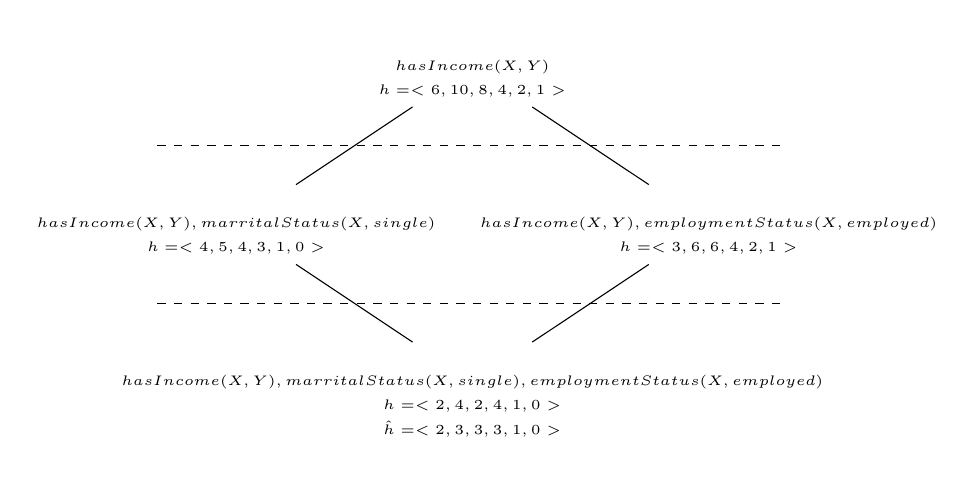
\begin{tikzpicture}
    [scale=1,auto=center,every node/.style={minimum size=1cm}]
      \node (p)[font=\tiny]   at (4,10) {$hasIncome(X,Y)$};      
      \node (n1)[font=\tiny]  at (1,8)  {$hasIncome(X,Y),marritalStatus(X,single)$};     
      \node (n2)[font=\tiny]  at (7,8)  {$hasIncome(X,Y),employmentStatus(X,employed)$}; 
      \node (n12)[font=\tiny] at (4,6){$hasIncome(X,Y),marritalStatus(X,single),employmentStatus(X,employed)$};

      \node (pd)[font=\tiny]   at (4,9.7)	 {$h=<6,10,8,4,2,1>$};
      \node (pd)[font=\tiny]   at (1,7.7)  	 {$h=<4,5,4,3,1,0>$};
      \node (pn2)[font=\tiny]  at (7,7.7)  	 {$h=<3,6,6,4,2,1>$};
      \node (pn12)[font=\tiny] at (4,5.7)  	 {$h=<2,4,2,4,1,0>$};
      \node (en12)[font=\tiny] at (4,5.4)  {$\hat{h}=<2,3,3,3,1,0>$};
  


      \foreach \from/\to in {p/n1,p/n2,n1/n12,n2/n12}
	\draw (\from) -- (\to);

      \draw[dashed] (0,9) -- (8,9);
      \draw[dashed] (0,7) -- (8,7);

      %\node (level0)[font=\small] at (10.5,10) {level $0$};
      %\node (level1)[font=\small] at (10.5,8)  {level $1$};
      %\node (level2)[font=\small] at (10.5,6)  {level $2$};
    \end{tikzpicture}
  \end{figure}

 \begin{center}
    $\chi^2=\sum_{i=1}^{k} \cfrac{(h_i - \hat{h_i})^2}{\hat{h_i}}=1 \quad \Rightarrow \quad $p-value$=0.96$
 \end{center}

 
\end{frame}
%-----------------------------------------------------------------------------------------------------------------------
\begin{frame}
\frametitle{Independence checks}
  \begin{itemize}
   \item  If there's not enough evidence of dependence, we assume independence, then: \\ \quad
      $x$ :- $p,y \equiv x$ :- $p$ \\ \quad
      $y$ :- $p,x \equiv y$ :- $p$
   \item The greater the $\chi^2$ value, the greater the evidence that $x$ and $y$ are dependent given $p$, therefore
the more interesting it is to join both $py$ and $px$
   \item As heuristics, we can prune a node when it's independent for all possible pairs of joining parents. That means
its not interesting to any of its parents.
  \end{itemize}
\end{frame}
%-----------------------------------------------------------------------------------------------------------------------
\begin{frame}
\frametitle{Search in the Lattice}
  In the refinement loop from the core-ILP, the clauses have a fixed head and literals are added to the body.
  In the following example, we would have $a$ as head literal, $r$ as root and $b$, $c$, $d$ as possible new
literals
 \begin{columns}[c]
  \column{0.75\textwidth}
    \begin{figure}
    \includegraphics[height=0.5\textheight]{./Figures/headmap}
    \end{figure}
  \column{0.25\textwidth}
      \begin{tabular}{r | l}
	a & b=$m_{a,rb}$ \\
	  & c=$m_{a,rc}$ \\
	  & d=$m_{a,rd}$
      \end{tabular}
 \end{columns} 
\end{frame}
%-----------------------------------------------------------------------------------------------------------------------
\begin{frame} 
\frametitle{Search in the Lattice}
   What has to be done?
  \begin{itemize}
   \item Search the node with body literals
   \item For each child of such node check head literal can be further added, if so collect the new literal and the
interestingness value of adding the head
   \item Sort the possible new literals by interestingness
  \end{itemize}
  Alternative?
  \begin{itemize}
   \item Create mapping in every node with the possible head literals as key and sorted literals to be added to body as
value, e.g. for the node $r a_1 b_1$ in the lattice example:
   \begin{center}
    \begin{tabular}{r | l}
      $a_1$ 	& $c_1$ [$m_{a_1 , r b_1 c_1}$] \\
		& $c_2$ [$m_{a_1 , r b_1 c_2}$] \\
      \hline
      $b_1$	& $c_1$ [$m_{b_1 , r a_1 c_1}$] \\
		& $c_2$ [$m_{b_1 , r a_1 c_2}$]
    \end{tabular}
   \end{center}
   \item Only add entry if head and new literal not independent given body
  \end{itemize}
\end{frame}
%-----------------------------------------------------------------------------------------------------------------------
\begin{frame}
  \frametitle{Incorporating the Lattice in the Core-ILP}
  In the refinement step, we detect clauses with body containing a lattice root
  \begin{itemize}
  \item If clause satisfies support threshold and does not satisfy confidence threshold
  \item Then search in lattice for body literals and head
  \item Check the interestingness of adding the head to the body and analyze whether to search for numerical intervals
  \item Query the lattice for suggestions of interesting literals to be added to the clause
  \end{itemize}
\end{frame}
%-----------------------------------------------------------------------------------------------------------------------
\section{Experiments}
%-----------------------------------------------------------------------------------------------------------------------
\begin{frame}
\frametitle{Experiments}
  Overall Settings:
  \begin{itemize}
   \item We compare 4 interestingness measures:
   \begin{enumerate}
    \item $supp$: Support Only
    \item $klsupp$: KL-divergence*Support
    \item $kldiv$: KL-divergence Only
    \item $jsdiv$: JS-divergence*Support
   \end{enumerate}
   \item Thresholds:
   \begin{itemize}
    \item $minConf=0.75$
    \item $minSupp=25$
    \item $minGain=1.25$
   \end{itemize}


  \end{itemize}

  $1^{st}$ Experiment: evaluation of the Correlation Lattice
  \begin{itemize}
   \item All data joined by person only (anonymized)
   \item All properties categorical (categories as literals)
   \item Create a lattice for $hasIncome$ property
  \end{itemize}
  $2^{nd}$ Experiment: evaluation of the ILP extension
  \begin{itemize}
   \item All data joined by person only (anonymized)
   \item All properties categorical (categories as literals)
   \item Not densely linked to other datasets
  \end{itemize}
\end{frame}
%-----------------------------------------------------------------------------------------------------------------------
\begin{frame}
\frametitle{Experiments}
 Compare interestingness measures:
 \begin{itemize}
  \item \begin{color}{red}divergence*support\end{color} vs. \begin{color}{blue}support only\end{color}
 \end{itemize}
 \begin{figure}
  \includegraphics[height=0.5\textheight]{./Figures/plots}
 \end{figure}
\end{frame}
%-----------------------------------------------------------------------------------------------------------------------
\begin{frame}
\Huge{\centerline{Thank you}}
\end{frame}
%----------------------------------------------------------------------------------------

\end{document} 